\chapter{Практическая часть}

Расчет нормального распределения можно вывести с помощью функции фунции NORMAL(RNj, m, $\sigma$), где RNj --- означает  порядковый номер датчика случайной величины, обычно от 1 до 7; m ---  математическое ожидание; $\sigma$ ---  среднее квадратичное отклонение.

В листинге 3.1 представлена реализация системы массового обслуживания на языке имитационного моделирования GPSS

\begin{lstlisting}[caption=Реализация системы массового обслуживания]
GENERATE (UNIFORM(1,1,5)),,,1000
Enqueue QUEUE QSystemQueue

SEIZE Operator
DEPART QSystemQueue

ADVANCE(NORMAL(1,9,2))
RELEASE Operator

TRANSFER 0.7,Complete,Enqueue 
Complete TERMINATE 1

START 1000
\end{lstlisting}

\clearpage

На рисунке 3.1 демонстрируется работа программы. Максимальная длина очереди при вероятности возврата заявки 70\% равна 896 заявки.

\begin{figure}[h]
	\centering
	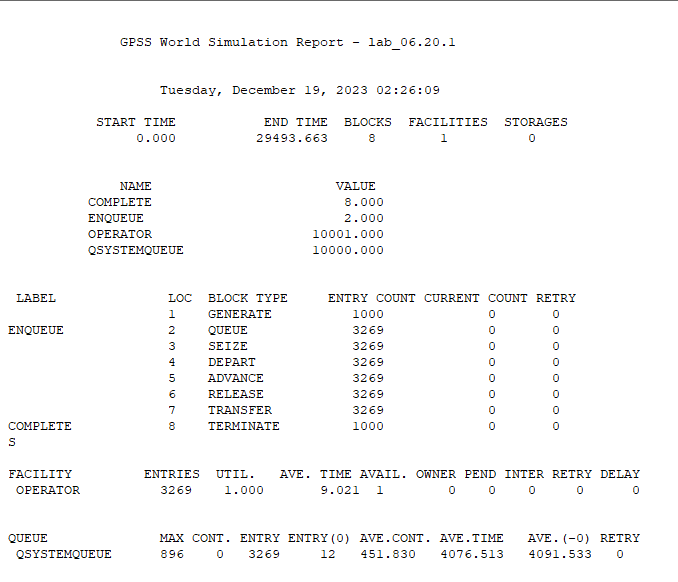
\includegraphics[height=0.55\textheight]{img/res.png}
	\caption{Отчёт системы массового обслуживания}
	\label{plt:even_comp_alg}
\end{figure}

